\chapter{Methodology}
\label{simulations}

Our evaluation methods are based on simulations using ns-3 \cite{ns3}, a discrete-event network simulator written in C++. ns-3 allows us to simulate the entire Internet stack, from physical links up through link, network, and transport level protocols. Developing our applications for ns-3 closely models the development process for a full implementation. We developed SCDTs and CNR at the ``application" level and ``install" them onto our simulated nodes. Our applications are written comparably to real implementations and behave similarly. Each instance of our software is separated from each other instance; just like in a real network, they can only communicate over the network using sockets. There is no overarching control program coordinating the nodes in the simulation for us or otherwise simplifying coordination and communication among nodes. The interfaces to the ns-3 library, such as our simulated sockets, closely parallel the actual C++ socket interfaces, meaning that porting application code from an ns-3 simulation into an actual implementation would not require major re-architecting.

ns-3 allows us to manually specify a network topology, including the number of nodes, the connections between them, the protocols used at each layer, and a number of parameters such as bandwidth, network delay, and packet drop rate. We use ns-3 library implementations of the IP stack including UDP and TCP; our code sits on top of these, handling the application-level SCDT/CNR protocols.  Both SCDTs and CNRs were coded in C++.  The advantage of this approach is that our simulated SCDTs closely mirror a full standalone implementation; the disadvantage is that trying new algorithms is non-trivial, and dealing with both ns-3's and C++'s nuances makes rapid prototyping more difficult.

\begin{figure}[h]
	\begin{center}
		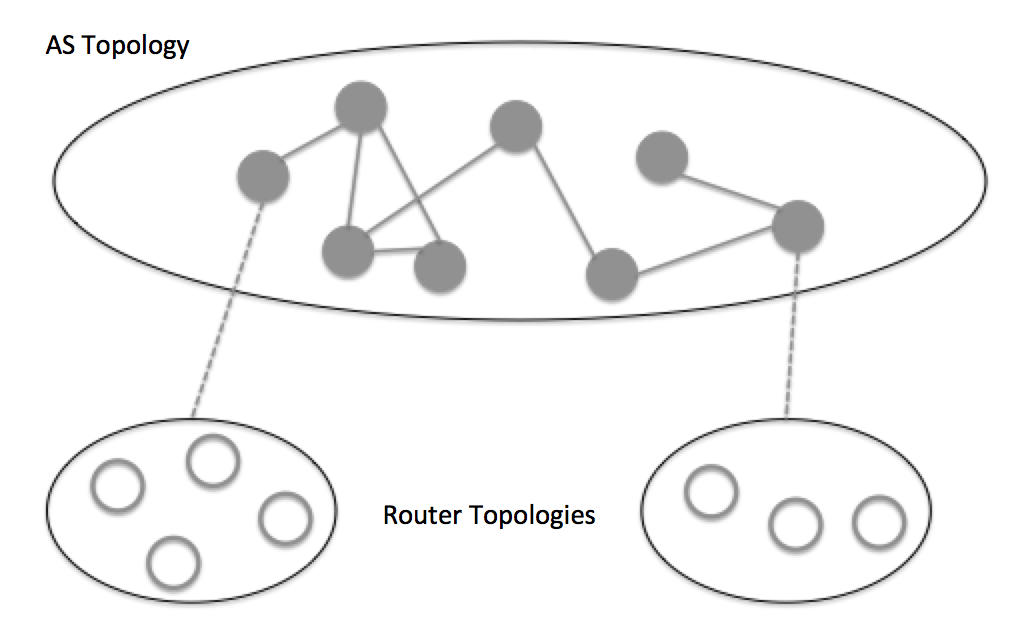
\includegraphics[scale=0.6]{brite.png}
	\end{center}
	\vspace{-1.3em}
	\caption{\small \itshape A diagram of a top-down BRITE topology \cite{brite-user}.}
	\vspace{-1em}
	\label{fig:brite}
\end{figure}

However, just because a given topology in ns-3 behaves as it would in the real world does not mean that the topologies selected necessarily reflect real-world deployments. To address this issue and avoid biasing our results by selecting hand-built topologies that favor our algorithms, we instead take advantage of BRITE \cite{brite} and BRITE integration in ns-3. BRITE, the Boston university Representative Internet Topology gEnerator, is a synthetic topology generation framework \cite{gtitm, inet} designed to create topologies that closely resemble the Internet in aspects including hierarchical structure and degree distribution. Using BRITE topologies for our simulations greatly strengthens our argument that SCDTs and CNR are practical in real-world deployments. BRITE offers a number of different models, which can be tuned to generate topologies with various numbers of ASes and nodes. Specifically, we configured BRITE to use a model composed of the the Barab{\'a}si-Albert model \cite{BA_model} and the Waxman model \cite{waxman} (see~\autoref{fig:brite}), which are algorithms for generating network topologies. BRITE also offers many tunable parameters to tweak how the model performs; see~\autoref{tab:brite-params} for more on BRITE parameters. 

\begin{table}
	\begin{center}
		\begin{tabular}{|c|c|}
			\hline
			\textbf{Parameter} & \textbf{Description} \\
			\hline
			\textbf{Flat Topology} & \\
			\hline
			\texttt{HS} & Size of one side of the plane \\
			\hline
			\texttt{LS} & Size of one side of a high-level square \\
			\hline
			\texttt{N} & Number of nodes \\
			\hline
			\texttt{Model} & Model ID \\
			\hline
			\texttt{alpha} & Waxman-specific exponent \\
			\hline
			\texttt{beta} & Waxman-specific exponent \\
			\hline
			\texttt{Node Placement} & How nodes are placed in the plane \\
			\hline
			\texttt{m} & Number of links per new node \\
			\hline
			\texttt{Growth Type} & How nodes join the topology \\
			\hline
			\texttt{BWdist} & Bandwidth assignment to links \\
			\hline
			\texttt{MaxBW} & Max link bandwidth value \\
			\hline
			\texttt{MinBW} & Min link bandwidth value \\
			\hline
			& \\
			\hline
			\textbf{Top-Down Hierarchical Topology} & \\
			\hline
			\texttt{Edge Connection} & Method for interconnecting router topologies \\
			\hline
			\texttt{Intra BWdist} & Intra-domain bandwidth assignment distribution \\
			\hline
			\texttt{Intra BWMax} & Max bandwidth values \\
			\hline
			\texttt{Intra BWMin} & Min bandwidth values \\
			\hline
			\texttt{Inter BWdist} & Inter-domain bandwidth assignment distribution \\
			\hline
			\texttt{Inter BWMax} & Max bandwidth values for inter-domain links \\
			\hline
			\texttt{Inter BWMin} & Min bandwidth values for inter-domain links \\
			\hline
		\end{tabular}
	\end{center}
	\caption{Selection of BRITE model parameters and their meanings \cite{brite-manual}.}
	\label{tab:brite-params}
\end{table}

In each test run, we randomly select a subset of BRITE-generated leaf nodes to attach a node with our software ``installed". In order to generate our results, we run our tests repeatedly in order to get results across many different BRITE-generated topologies and many different distributions of overlay-enabled routers. We then draw our results from the aggregate of this data, arguing that it is representative of an average use case of SCDTs and CNR on the Internet.